\documentclass[11pt,letterpaper]{article}
\usepackage[margin=0.92in]{geometry}
\usepackage[T1]{fontenc}
\usepackage{lmodern}
\usepackage{microtype}
\usepackage{setspace}
\usepackage{booktabs}
\usepackage{tabularx}
\usepackage{array}
\usepackage{amsmath,amssymb}
\usepackage{enumitem}
\usepackage{graphicx}
\usepackage{float}
\usepackage{xcolor}
\usepackage{hyperref}
\usepackage[numbers,sort&compress]{natbib}
\usepackage{tikz}
\usetikzlibrary{arrows.meta,positioning,shapes.geometric}
\definecolor{ink}{HTML}{142B3B}
\definecolor{accent}{HTML}{177F83}
\definecolor{muted}{HTML}{546874}
\hypersetup{colorlinks=true,linkcolor=ink,citecolor=accent,urlcolor=accent,pdftitle={Lamina: Source-aware production methods for document workflows},pdfauthor={Lamina Project}}
\setstretch{1.09}
\setlength{\parskip}{0.33em}
\setlength{\parindent}{0pt}
\setlist{nosep,topsep=0.25em,leftmargin=1.5em}
\title{\vspace{-1.1em}\textbf{Lamina}\,\\[0.2em]\large Source-aware production methods for document workflows}
\author{Lamina Project}
\date{21 September 2026 --- technical design and implementation status}
\begin{document}
\maketitle
\vspace{-1.4em}
\begin{abstract}
Teams increasingly ask language models to turn large, changing source collections into guides, briefs, references, questions, and other deliverables. A model can read and write, but an operational workflow must still decide which sources have authority, what information must survive compression, which workers require shared context, what can run concurrently, and what must be repaired after a source or review finding changes. Lamina is open-source infrastructure for these decisions. It now includes a source-linked guide builder, a separate reusable method runtime, and a source-aware production engine connected to a local project interface, CLI, exports, and persisted recovery. Source-role selection, blind checks on assessment runs and optional local PCM audio rendering close narrower boundaries of that path. This paper defines a broader task-shaped architecture without assuming that every output is a lesson or that a dependency graph alone is the method. It gives operational definitions for source ownership, context selection, dependency and resource edges, cache identity, and bounded repair. A local synthetic benchmark demonstrates scheduler and cache behavior only; semantic quality, production latency, and competitive advantage require a new-source, quality-matched evaluation. The main product hypothesis is that an inspectable source-to-decision-to-artifact trail can reduce the work of producing and safely updating useful documents. That hypothesis is not yet established by the present fixtures.
\end{abstract}

\section{The production problem}
A team preparing an operating brief may have a current procedure, a superseded note, a table of exceptions, and a prior document used only as a style example. It needs a result that can be used, not a plausible summary. A single model call can blend the old and new rules, lose a condition in a table, or write a clean draft whose source basis is hard to revise. Sending the whole collection to every writer increases input cost and still does not ensure that the critical condition is attended to; long-context retrieval is known to vary with position and task \cite{liu2024lost}. The failure may originate before writing, when a parser, reader, or planner narrows what later workers are allowed to see.

The customer value is clearest after change. If a rule or document is revised, the owner must know what the earlier artifact depended on, which decisions are invalid, what can be reused, and whether the replacement reached the intended surface. Recreating the entire document is expensive and can introduce unrelated errors. Editing the final sentence alone can leave a false upstream interpretation available for the next release. Lamina's intended unit of work is therefore a \emph{production method}: an explicit, inspectable way to transform a defined source set into a defined artifact, with decisions and repair paths retained.

This is neither a claim that graphs or parallel agents are new nor a claim that bookkeeping can replace editorial judgment. Parallel function execution has been studied in LLM systems \cite{kim2024llmcompiler}; graph-based agent workflows, durable state, and interruptions are available in established tools \cite{langgraph2026,googleadk2026}. The distinct question here is whether a source-aware production contract and a record of semantic decisions make document change and repair less costly at matched output quality. That question requires testing.

\section{Evidence from several output forms}
Lamina's design was informed by document and learning-product work with incompatible output contracts. A differential reference must own each retrieval target, preserve meaningful variants, and make the answer to a presenting problem easy to find. A spoken lesson must preserve lists, explanation, useful repetition, and actual playable delivery. An interactive case must keep candidate-visible findings separate from an examiner's answers and reveal new information after actions or elapsed time. A written case generator adds a separate setter, question-specific answer keys, and a blind solver that sees only the staged information available to a candidate at each turn. A technical brief needs a defensible argument and a record of conflicting sources. They can share infrastructure for sources, work allocation, provenance, and revision, but they should not share one mandatory narrative template.

Three distinctions recur across these jobs. First, \emph{source consideration} is not final coverage: a model may read an item and correctly omit it, or may never see an item that it later claims to have considered. Second, a source quotation is evidence of provenance, not proof that the sentence citing it is entailed, correct, or useful. Third, an artifact's schema and its user experience are separate: a valid script is not a verified recording; a well-formed case is not necessarily a realistic encounter; a PDF's page count does not establish that its diagrams are legible. These distinctions determine what receipts and tests are needed at each boundary.

\section{A task contract before a graph}
A job begins with a task contract
\begin{equation}
\mathcal{T}=(G,A,S,P,O,Q,R),
\label{eq:contract}
\end{equation}
where $G$ is the goal, $A$ the audience or operator, $S$ the accepted source set, $P$ the policy governing each source's use, $O$ the target artifact and its delivery surface, $Q$ the acceptance criteria, and $R$ the time, model, money, context, and machine-resource limits. This is an engineering interface, not a formula that scores document quality. If any component is missing, a method may still run, but its success claim is correspondingly weaker.

Source policy is more precise than a generic `included' flag. A current specification may establish an operational rule; an old note may document a conflict but lack present authority; a style exemplar may influence tone but not factual claims; held-out questions must remain out of generation prompts. Lamina now accepts an operator-assigned policy for each selected teaching source: authority, supplement, historical, or form exemplar. Factual sources enter reading and evidence; form exemplars enter a bounded form-only context. Held-out assessment sources remain excluded. These roles are enforced at the input boundary, although model compliance with authority distinctions and stylistic influence still requires review. A source has an identity, version or hash, role, and locator. A later change in policy is a semantic input change even when the underlying file bytes are unchanged.

An assessment question can legitimately serve as an example of \emph{question form} while being prohibited as factual teaching evidence. Another question can be protected as a held-out evaluation item. These roles cannot be inferred from a filename. A manifest should distinguish sources discovered, inventoried, actually read, selected as factual evidence, used as form exemplars, and withheld. A source count at one boundary must not be reported as comprehensive use at another.

The intended representation follows the task. For a guide it may be claims, conditions, exceptions, causal steps, and contrasts. For a differential reference it may be presentation--answer objects with one owner per retrieval target and distinct variants when the question genuinely changes. For an interactive case it may be states, candidate requests, released findings, actions, consequences, and marking opportunities. Figure and table regions require modality-aware extraction and verification. The general rule is to choose a representation that preserves the distinctions needed to judge the final artifact. A universal `concept' type is convenient but can hide the answer unit or behavior that actually matters.

This also changes review. A document claim may be reviewed for support and contradiction. A differential object needs its answer family, exclusions, qualifiers, and retrieval target checked. An interactive case requires a state-machine review: can the candidate obtain an indicated finding, does a treatment alter the next observation, and does the examiner possess the data required to answer reasonable questions? A single generic `pass' score collapses these into an unhelpful average. The method should declare the domain of each check and whether failure blocks delivery, creates a review flag, or opens a source-policy decision. A model reviewer can help find defects; its response is not an independent authority over a clinical, legal, or financial claim.

A model can propose objects and relations, while code owns stable IDs, source locators, exact membership, and declared limits. Relations such as \emph{same target}, \emph{variant}, \emph{contrast}, \emph{prerequisite}, and \emph{conflict} should be typed rather than collapsed into a single semantic merge. An ambiguous merge should remain unresolved for review. A selected object can be written, deferred, deliberately omitted, or left open; no universal rule should force all source items into prose. The acceptance criteria decide how much omission accounting is justified by the task.

Two limits prevent this representation from becoming a decorative ontology. An object must have a downstream consumer: a writer needs it to explain, a reviewer needs it to test, or a repair operation needs it to locate a decision. If no consumer uses an added field, it should not be required. Likewise, exact structural accounting should be paired with a semantic counterexample. A validator can prove that every extracted item has an owner while a merged item silently loses an exception. A source-bound object ledger should therefore expose the original region and the model's claimed transformation, allowing an independent reviewer to sample risky merges and central answers rather than trusting item counts.

\section{Source windows and ownership}
Reading a large source requires bounded packets, but a boundary can split a definition from its condition. Let the accepted regions be $S_1,\ldots,S_n$. A reading job $j$ receives a focal core $C_j$ and neighboring context $H_j$. The reader may use the halo to interpret the core but owns extraction only from $C_j$. For an exact partition of readable core regions,
\begin{equation}
\bigcup_j C_j=S_{\mathrm{readable}},\qquad C_j\cap C_k=\varnothing\ \text{for }j\neq k.
\label{eq:core}
\end{equation}
This ownership rule prevents the same boundary material from becoming duplicate findings merely because it appeared in two windows. It is a structural invariant, not a completeness claim: an unreadable figure, a broken table order, or a reader's missed clause still requires separate detection. A region inventory should label what was parsed, unsupported, or reopened from the original page.

The useful window size is not simply the largest context a model will accept. Small windows reduce per-call cost but can remove distant qualifiers; large windows can crowd the relevant passage and cause repeated work. A source-aware method should vary core size, halo width, and bridge review with source topology and task. It should preserve exact source IDs and short supporting spans for consequential statements. A writer need not receive every full source if a shared plan and local evidence packet carry the needed material, but a reviewer diagnosing an omission should be able to reopen the uncompressed source.

\section{Methods and execution semantics}
A method is a versioned proposal for how to do the job. It names its applicability conditions and exclusions, expected artifacts, worker roles, data passed to them, dependencies, resource limits, and review policy. It must be possible to reject the method for a task whose source modality or acceptance criterion it cannot handle. Current Lamina method files declare a bounded JSON graph and run through an operator-configured adapter. They do not select themselves, revise themselves, or inherit every source check from the guide builder.

Let $V$ be the jobs of a run. Distinguish at least four relationships:
\begin{itemize}
\item A \emph{hard-result edge} $u\rightarrow v$ means $v$ waits for and receives $u$'s completed result.
\item A \emph{shared-plan relation} means two jobs use the same versioned map or editorial decision, without requiring one writer's finished prose.
\item An \emph{evidence-validity relation} links a source region or semantic decision to work that must be reconsidered if it changes; it does not automatically mean every descendant must be regenerated.
\item A \emph{resource relation} assigns work to a model, parser, renderer, review, or other lane with finite capacity. It can delay work without adding semantic information.
\end{itemize}
One untyped `depends on' list cannot express all four without over-serializing or under-invalidating work. The current generic method runtime implements hard-result edges and resource lanes. The source-aware production path uses parallel local reading, a shared route, parallel sections, and review, but its plan is not previously finished prose. This distinction matters for callbacks and duplicated explanations: some writers need the shared plan and exact previous evidence; others genuinely need a prior finished section. Both patterns should remain available and be compared on the same task.

A source-aware planner should present alternative decompositions when evidence is weak. A source-order route retains local sequence and can be cheap for a short, coherent file. A shared topic board can coordinate parallel sections across multiple overlapping files, but its global reconciliation call may dominate latency or erase a distinction. A dependency chain of finished sections can improve continuity and exact callbacks, but it serializes writing and expands later context. A cross-section editor over parallel drafts can preserve overlap while paying an additional review and repair cost. The planner's choice should cite task conditions---source topology, output form, conflict density, context budget, and delivery deadline---rather than merely selecting the strategy with the most nodes. Keeping rejected alternatives visible makes later repair intelligible: a failed source-order result may call for a different representation, not another prompt sentence.

\begin{figure}[t]
\centering
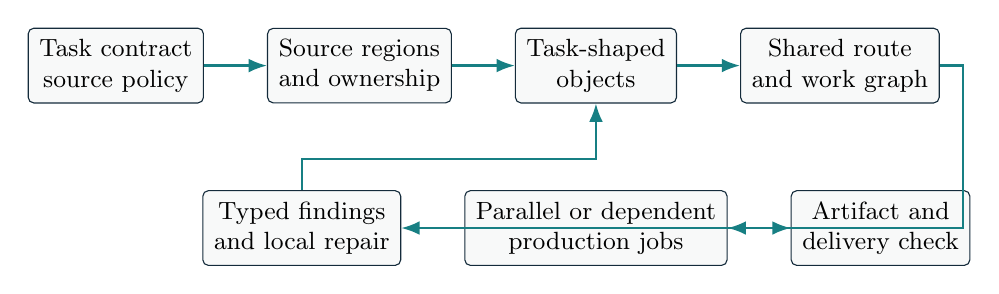
\begin{tikzpicture}[>=Latex, node distance=7mm and 8mm, every node/.style={font=\small}, box/.style={draw=ink,rounded corners=2pt,fill=ink!3,minimum height=8mm,align=center,inner sep=4pt}, line/.style={->,thick,draw=accent}]
\node[box] (task) {Task contract\\source policy};
\node[box,right=of task] (regions) {Source regions\\and ownership};
\node[box,right=of regions] (objects) {Task-shaped\\objects};
\node[box,right=of objects] (route) {Shared route\\and work graph};
\node[box,below=11mm of objects] (writers) {Parallel or dependent\\production jobs};
\node[box,left=of writers] (review) {Typed findings\\and local repair};
\node[box,right=of writers] (delivery) {Artifact and\\delivery check};
\draw[line] (task)--(regions); \draw[line] (regions)--(objects); \draw[line] (objects)--(route);
\draw[line] (route.east) -- ++(3mm,0) |- (writers.east);
\draw[line] (writers)--(delivery); \draw[line] (delivery.west) -- ++(-3mm,0) |- (review.east);
\draw[line] (review.north) -- ++(0,4mm) -| (objects.south);
\end{tikzpicture}
\caption{Intended source-aware production loop. The diagram separates semantic decisions from scheduling and delivery. Review may reopen a specific object or source decision; it need not restart every job. The fully connected loop is a design target, not a claim that all boxes are automated in the current release.}
\label{fig:flow}
\end{figure}

\section{Context assembly as an explicit decision}
A worker's context is selected, not inherited indiscriminately. Let $I_v$ be the candidate items for job $v$ and $P_v\subseteq I_v$ the protected items required by the task or a consequential claim. Each item $i$ has measured size $b_i$ in the adapter's tokenizer. If the available input budget after instructions and output reserve is $B_v$, assembly chooses $X_v\subseteq I_v$ such that
\begin{equation}
P_v\subseteq X_v,\qquad \sum_{i\in X_v} b_i\leq B_v.
\label{eq:context}
\end{equation}
A relevance score can rank optional items, but it is not a safety guarantee. If the protected set alone exceeds the budget, the job should split or ask for a scope decision; silent truncation violates the contract. Each packet should record the plan version, source and object IDs included, omitted candidate counts, and actual request size. The reviewer may need access to a broader inventory than a writer, precisely because a narrowed author packet cannot reveal what was lost before authoring.

The context-amplification ratio
\begin{equation}
A=\frac{\sum_{v\in V}\operatorname{inputTokens}(v)}{\operatorname{tokens}(\text{distinct accepted source text})}
\label{eq:amplification}
\end{equation}
is descriptive rather than an optimization target. Repeating a short protected rule across writers can prevent an error; duplicating an entire corpus in each local call can waste cost and attention. Report $A$ by stage and alongside the largest request, source coverage, and accepted artifact quality. A low ratio achieved by starving workers of necessary context is not an improvement. The current method runner can select top-level task fields and direct dependency results; it does not yet implement the source-aware constrained selection in Eq.~\ref{eq:context}.

\section{Concurrency and measured resource limits}
For job service times $t_v$, total service work $W=\sum_v t_v$ and longest hard-dependency path $D$, the ideal lower bound on elapsed service time with $p$ equivalent workers is
\begin{equation}
T\geq\max\left(D,\frac{W}{p}\right).
\label{eq:workspan}
\end{equation}
If lane $r$ has capacity $c_r$ and jobs using it require total lane service $W_r$, then a resource-aware lower bound is
\begin{equation}
T\geq\max\left(D,\frac{W}{p},\max_r\frac{W_r}{c_r}\right).
\label{eq:lanebound}
\end{equation}
These are classical work/span and capacity arguments, not new Lamina theorems; scheduling analyses such as work stealing assume particular task structures and costs \cite{blumofe1999scheduling}. Equation~\ref{eq:lanebound} assumes compatible service-time units and does not model simultaneous resource demands, provider throttling, request setup, queue wait, human review, retries, or delivery. It should locate possible bottlenecks, not predict a wall-clock completion time.

The design choice is where to put genuine dependency. Adding parallel writers cannot remove a long global reconciliation call from $D$. Requiring every writer to wait for completed earlier prose increases $D$, though it may lower duplication and repair. Resource contention can nullify a wider worker pool: a speech renderer and transcript checker sharing one memory-bound accelerator may be effectively serial even when model writers overlap. A finite batch graph does not necessarily meet the steady-state assumptions of a simple queueing formula. Instrument enqueue, start and end times, lane occupancy, retries and tail latency before using such a model.

A checked-in local benchmark exercises an older fixed graph of 24 simulated extraction jobs, two global steps, and six simulated author/review pairs. Its handlers only sleep and return tiny JSON objects. At worker limits 1, 4 and 8, cold wall times were 2.412, 0.865 and 0.595 seconds, respectively; warm cached runs took about 0.018--0.022 seconds with no handler calls. These measurements show scheduler overlap and cache reuse on one machine under artificial delays. They provide no evidence of model throughput, document quality, media delivery, or a general speed advantage. A separate integrated-path measurement is required after its implementation is frozen.

A second checked-in scheduler benchmark uses the same real SQLite/cache execution substrate with 64 sleep-only reading jobs, two serial global jobs and 16 sleep-only author/review chains, for 98 handler calls. Table~\ref{tab:widths} reports one local run per width, not a sampling distribution. The 32-worker setting reached 30 simultaneous handlers, not 32; the global stages and paired author/review dependencies limit overlap. Warm runs made zero handler calls but had non-monotone wall times as thread and cache bookkeeping remained. These measurements establish that configured width changes overlap under this fixture, not that a wider setting improves an inference workload.

\begin{table}[tbp]
\centering
\small
\begin{tabular}{@{}rrrrr@{}}
\toprule
Worker cap & Cold wall (s) & Peak handlers & Warm wall (s) & Warm calls \\
\midrule
1 & 6.001 & 1 & 0.054 & 0 \\
4 & 1.690 & 4 & 0.020 & 0 \\
16 & 0.777 & 16 & 0.082 & 0 \\
32 & 0.626 & 30 & 0.136 & 0 \\
\bottomrule
\end{tabular}
\caption{Synthetic sleep workload on one local machine (Darwin arm64, Python 3.14.7, SQLite 3.53.4); one cold and one warm run per width. No model, human review, figure parsing or media delivery is in these times. Source: \texttt{benchmarks/results/production-widths.json}.}
\label{tab:widths}
\end{table}

\section{Cache identity, review, and repair}
A reusable job result must be keyed by its actual semantic request: source and policy versions, the job's instructions and selected task fields, relevant dependency outputs, adapter identity, and any selected operator observation. Changing a label or an unrelated branch should not discard sound work; changing the source meaning or reviewer policy should not silently reuse an obsolete result. A content-addressed job store can make reuse explicit, but cache hits are not quality judgments. A stale reviewer verdict is especially dangerous when the artifact or source version it examined changes.

A review result should name the affected object and observed defect, not merely return `revise'. Examples include unreadable source region, missing answer object, false merge, unsupported claim, wrong condition, broken cross-section reference, candidate-answer leakage, and delivery failure. The finding needs an artifact location, source link, severity, reviewer identity, and exact artifact revision. Then the system can decide whether to reopen parsing, representation, selection, a writer, a renderer, or publication. Some findings need a human authority decision; a model should not resolve contradictory sources by confidence alone.

The dependency closure of a changed node is a candidate recheck set, not the exact repair bill. Let a repair receipt be
\begin{equation}
R(o)=(s_o,m_o,h_o,d_o),
\label{eq:repair}
\end{equation}
where $s_o$ is re-executed service seconds, $m_o$ reported model or external charges, $h_o$ human review minutes, and $d_o$ replacement-delivery count for observation $o$. These values are deliberately not summed without an explicit conversion rule. A smaller invalidation set is useful only if the final artifact remains correct. Lamina currently caches stages and generic method nodes; the fixed guide can block export on review failure; and the production path can target a named section for revision, with a bounded section repair and re-review. Typed finding-to-upstream-cause routing and independent verification of final semantic quality remain limited; a generated repair is not automatically proof that its issue was fixed.

\section{Experience and method reuse}
Operational reuse and methodological learning are different. Operational reuse retrieves a node result whose semantic inputs are unchanged. Methodological learning changes a future decision: source policy, representation, window size, work graph, context packet, reviewer, or output form. Lamina's method runtime stores run receipts and operator observations. An operator can explicitly attach a same-family observation ID to a later node, and that observation then enters the node's context. This is a real downstream consumer of stored feedback. It is not automatic method selection or evidence that the observation improved the output.

A method revision should be a testable hypothesis: what failure it addresses, what it changes, what it preserves, and what new cost it may impose. Compare old and new versions on source collections not used during tuning, with an explicit counterexample where the favored method could fail. Record losses as well as gains. Systems such as DSPy already study metric-driven optimization of language-model pipelines \cite{khattab2024dspy}; Lamina should not claim that optimizing prompts or saving reusable methods is novel. Its narrower research question is whether task-specific source and repair decisions improve accepted document production under realistic change.

\section{Worked example: a disputed timeout}
Consider a fictional engineering team preparing a short export-worker brief. Its owner-designated current specification says a worker receives a 90-second lease, renews it every 30 seconds while healthy, and stops producing output if renewal fails. It says the scheduler may reassign a job only after lease expiry. A historical runbook says operators once expected a 60-second timeout and records an incident in which a second worker began while the first appeared still to write. The runbook does not establish which timeout was configured during that incident or whether partial output was cleaned up. The team asks what to check before changing its retry timer.

A source-order summary could repeat both timeout numbers without explaining authority. A reader that aggressively merges them could produce one false rule. An evidence-led method instead gives each source an independent reader. The readers preserve atomic claims, short excerpts, source IDs and conditions. A reconciliation job applies the task owner's authority policy, retains the old instruction as historical and the incident as an observation with unresolved cause, and produces a shared evidence board. A behavior writer and an operations writer use that same board in parallel. Their reviewer receives both drafts \emph{and} the board, then flags a lost qualifier or unsupported recommendation. This is the repository's portable six-node technical-brief example; the graph and context wiring have been structurally validated, but no model-written brief from that example has been independently accepted as an engineering answer.

Suppose the current specification changes its lease duration. The reader of that source and the reconciliation board are invalidated. Both writers may need fresh context, even if only one section visibly mentions the number. The historical reader can remain reusable if its selected task and source text are unchanged. A review finding about cleanup may instead target an information gap: the current specification is silent, and no amount of rewording should fabricate an answer. A good final brief should state the gap and recommend checking the actual cleanup contract. The repair trace should identify the new source version, reopened decisions, executed and reused jobs, reviewer result, and exact delivered brief. The present example demonstrates graph structure and local receipts, not that full conflict-to-delivery loop.

A separate deterministic production fixture exercises the actual source-aware engine with two original short source files and three planned sections. Its initial run reports one flagged section, one repair call, and no remaining flagged sections. On a named revision to section three, six of eight stage requests are cache hits; only section three's write and review are misses, and the other two section bodies remain byte-identical. This tests request identity, targeted rerun and trace structure. The provider in this fixture returns canned JSON, so it cannot show that an LLM resolved the timeout conflict, wrote a useful brief or improved after review. The fixture's millisecond timings are not production latency measurements.

\section{Current implementation and boundary}
The repository has three related but unequal paths. The fixed guide builder ingests Markdown, text and extractable PDF text; stores source hashes, ordered units and locators; extracts with a short adjacent halo; globally reconciles and plans; authors and reviews lessons; and exports source-linked reading material. Validation checks certain source ownership, quotation, membership and output-shape properties. It cannot prove that parsing recovered visual meaning, that extraction found every important object, or that a citation entails an authored sentence. Its planned route and prerequisite evidence do not equal completed earlier prose.

\begin{table}[H]
\centering
\small
\begin{tabularx}{\linewidth}{@{}>{\raggedright\arraybackslash}p{0.22\linewidth}>{\raggedright\arraybackslash}X>{\raggedright\arraybackslash}p{0.29\linewidth}@{}}
\toprule
Capability & Present mechanism & Status boundary \\
\midrule
Source identity and policy & Hashes, ordered units, locators, authority/supplement/historical/form roles & Working for supported text; model's use of authority still needs review \\
Fixed guide & Extract, reconcile, plan, author, review and export & Working application; one teaching route \\
Reusable method & User-declared JSON jobs, dependencies, lanes, cache and receipts & Working separately; semantic output rules external \\
Source-aware production & Bounded reading, shared route, section production and revision & Working local engine/API/CLI; semantic quality unproven \\
Retrieval targets & Opt-in guide/assessment catalog partitions extracted ideas into source-backed prompts and answer groups & Structural ownership checked; semantic equivalence unproven \\
Assessment check & Every assessment runs candidate-only solve, then separate judge with key and exact excerpts & Working local stage; no interactive administration or provider-memory guarantee \\
Audio delivery & Optional command adapter, PCM WAV check, hashes and local render lock & Working local file verification; no listened or ASR quality check \\
Experience & Operator-selected observations enter named future nodes & Explicit reuse; no automatic adaptation \\
Local delivery and recovery & HTML, Markdown, optional PDF, report, plan and project resume & Working locally; external publication separate \\
Typed upstream repair & Finding-to-cause routing across source, representation and output & Design target beyond section repair \\
\bottomrule
\end{tabularx}
\caption{Status distinctions in the current checkout. Local end-to-end wiring and deterministic tests establish mechanics; they do not establish human-accepted model quality.}
\label{tab:status}
\end{table}

The generic method runtime executes data-only JSON nodes with hard dependencies, task-field selection, worker and lane capacities, cache receipts, and operator-selected observations. Its generic response check requires a JSON object; declared expected shapes are hints, not fully enforced semantic contracts. The source-aware production engine reads selected factual teaching sources in bounded, owned windows with full neighboring units, passes bounded form exemplars separately, asks a model for a natural section route and a representation per section, then writes and reviews sections under separate concurrency limits. For a guide or assessment, an opt-in retrieval stage assigns every extracted idea to one canonical question or use context with source-exact answer items. Related targets can remain variants. Assigned targets and answer items reach the guide or examiner artifact; deliberate omissions and reasons remain in the plan and report. This does not verify that semantic merging was wise or that extraction was complete. One material review finding can trigger a section-local repair and re-review; unresolved findings remain visible. A named revision changes the selected section request and reuses unchanged cached work. The local project API persists state, marks unfinished work interrupted after restart, and can resume from retained plans and cache. The CLI and local Projects interface call the same engine. Export writes Markdown, HTML, a report, plan and optional PDF; assessment export separates candidate and examiner files. Candidate-facing exports omit private answer and planned section titles. Every assessment run asks a provider to answer each candidate section using only that section and prior candidate bodies; a separate judge call then receives the blind answer, marking text and exact cited excerpts. The boundary separates call inputs, not hidden provider state, and a model finding is not a proof of answerability. An optional audio adapter renders a ready podcast script to PCM WAV, checks format, duration and file hashes, and records the text submitted for synthesis. A per-local-user process-safe file lock serializes uncached adapter invocations, while cache hits skip it. This establishes a playable technical file, not pronunciation, transcript fidelity, or a listener's acceptance. These mechanisms are implemented and structurally tested. They do not automatically infer prose-section dependencies after a revision, interpret arbitrary figures, administer a live oral case, or prove audio or clinical quality. The generic method graph remains a separate execution path rather than replacing the production engine.

\section{Evaluation and competitive position}
The fair comparison is time and total cost to a \emph{quality-matched accepted artifact}, including operator work. Freeze a new permissioned corpus and task contract before running. Include a difficult region such as a table or figure, overlap, one contradiction, and at least one known omission risk. Independent reviewers inventory important source objects, conditions and acceptable deliberate omissions from the rendered originals; preserve their disagreements. Hold any evaluation questions out of generation. Compare Lamina with a careful source-order baseline and, where feasible, fully configured external products under the same source and output rules. For an internal runtime comparison, keep the model/provider fixed; across products, report the combined system result rather than attributing a difference to orchestration alone.

Record first useful draft and accepted accessible artifact times, source-object misses and false merges, unsupported claims, editorial usability, model tokens, actual provider charges where available, human review minutes, retries, failed attempts and delivery checks. Distinguish estimated API-equivalent cost from observed incremental charge. Repeat paired tasks with rotated order and report median, tails, range and sample size. Then change one source, seed one local and one global finding, and ask a fresh operator to diagnose, repair and deliver again. Audit whether the smaller repair set was actually safe. A fresh-agent transfer run tests whether the saved method is usable without the original author. Structural tests, synthetic sleeps and a single polished example cannot establish semantic superiority.

Other products already provide capabilities adjacent to this design. Manus documents wide research and project context that evolves across tasks \cite{manus2026,manusprojects2026}. NotebookLM provides source-based audio generation \cite{notebooklm2026}. LangGraph and Google's ADK support graph workflows; ADK's newer documentation explicitly includes flexible graph and dynamic workflows \cite{langgraph2026,googleadk2026}. Product documentation does not disclose every internal mechanism, so Lamina should neither imply those systems lack graphs, memory or parallel research nor promise broad superiority. The plausible differentiated test is whether an operator can explain and revise a particular source-to-artifact decision with less accepted-work loss and less total effort. That remains a hypothesis.

\section{Conclusion}
A model is useful for reading, deciding, and writing; code is useful for exact identity, ownership, limits, scheduling, persistence and receipts. Neither can impersonate the other. Lamina's engineering direction is to make the decisions between source and delivered artifact explicit enough to coordinate workers, preserve meaningful alternatives, and repair the right work after change. The guide, method and source-aware production paths now establish different pieces of this substrate, with local project delivery and recovery attached to production. Policy-aware selection, blind assessment checks and optional PCM rendering close specific boundaries, while visual fidelity, live case behavior, upstream finding repair, listened audio verification and comparative semantic quality remain open. The next milestone is a new-source demonstration with an actual correction and a measured accepted artifact, not a larger graph or a stronger claim.

\bibliographystyle{plainnat}
\begingroup
\small
\setlength{\bibsep}{0.12em}
\bibliography{references}
\endgroup
\end{document}
